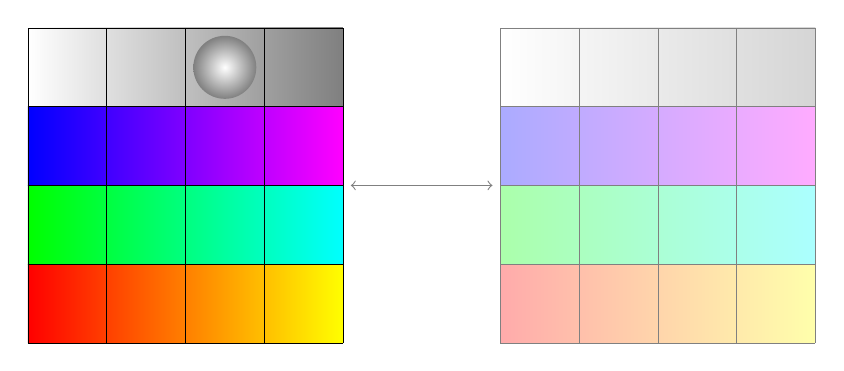
\begin{tikzpicture} 
  % Patch gradients
  \shade[left color=red,right color=yellow] (0,0) rectangle (4,1);
  \shade[left color=green,right color=cyan] (0,1) rectangle (4,2);
  \shade[left color=blue,right color=magenta] (0,2) rectangle (4,3);
  \shade[left color=white,right color=gray] (0,3) rectangle (4,4);
  %
  \shade[left color=red!33!white,right color=yellow!33!white] (6,0) rectangle (10,1);
  \shade[left color=green!33!white,right color=cyan!33!white] (6,1) rectangle (10,2);
  \shade[left color=blue!33!white,right color=magenta!33!white] (6,2) rectangle (10,3);
  \shade[left color=white!33!white,right color=gray!33!white] (6,3) rectangle (10,4);
  % Species gradients
  \shade[inner color=white,outer color=gray] (2.5,3.5) circle (0.4 cm);
  % Grids
  \draw[step=1cm,black,very thin] (0,0) grid ( 4,4); 
  \draw[step=1cm,gray,very thin] (6,0) grid (10,4); 
  % Arrows
  \draw[<->,gray] (4+0.1,2) -- (5,2) node[anchor=south] {} -- (6-0.1,2);
\end{tikzpicture}